\documentclass[a4paper,fleqn,review,12pt]{cas-sc}

\usepackage[numbers,sort&compress]{natbib}
\usepackage{amsmath,amssymb,bm}
\usepackage{graphicx}
\usepackage{booktabs}
\usepackage{xcolor}
\usepackage{xurl}
\usepackage{tikz}
\usetikzlibrary{arrows.meta,positioning,calc}
\usepackage{lineno}
\usepackage{needspace}

\graphicspath{{submit_figure/}}
\hypersetup{hidelinks}
\setcounter{secnumdepth}{3}
\setlength{\emergencystretch}{2em}
\interdisplaylinepenalty=10000
\predisplaypenalty=10000
\postdisplaypenalty=10000
\pretocmd{\subsection}{\Needspace{5\baselineskip}}{}{}
\AddToHook{env/thebibliography/begin}{\interlinepenalty=10000}
\numberwithin{equation}{section}

% Revisions dated 2026-09-06 are marked in red; the source manuscript is preserved.
\newcommand{\rev}[1]{{\color{red}#1}}
\newcommand{\todo}[1]{\textcolor{red}{\textbf{[TODO: #1]}}}

\begin{document}
\let\WriteBookmarks\relax
\def\floatpagepagefraction{1}
\def\textpagefraction{.001}

\title[mode=title]{On Craig--Bampton Model Reduction for Multi-Degree-of-Freedom Coupled Real-Time Hybrid Simulation}

\author{Ning Li}
\author{Yu Liang}
% Affiliations, e-mail addresses, and the corresponding author were not supplied in temp.tex.

\begin{abstract}[]
\rev{Limited actuation channels motivate the condensation of interface degrees of freedom (DOFs) in multi-degree-of-freedom real-time hybrid simulation (RTHS). This study examines the accuracy of static and Craig--Bampton reductions and formulates a channel-specific delay model with CR integration and linear quadratic regulator feedback. Two coordinate selections associated with divisions of a three-storey frame are evaluated. The delay-free benchmark uses whole-structure reductions with six and five retained physical coordinates, respectively; Craig--Bampton enrichment adds three fixed-interface modal coordinates. Its maximum relative error in the first two natural frequencies is 0.284\%, and its first-storey displacement normalized root mean square error reaches 0.138\% over the earthquake record and evaluated chirp bands, using the full-record response range for normalization. For the static model that condenses the middle-storey horizontal DOF, the corresponding maxima are 30.574\% and 26.858\%. The reported stability boundaries place Craig--Bampton above the static model in both divisions. A signed modal-share index describes changes at the actuated coordinates, while admissible delays are assessed through the closed-loop poles. The results show the accuracy gained by retaining internal modal dynamics and identify the model and feedback definitions required for delay-dependent comparison.}

\end{abstract}

\begin{keywords}
	\raggedright
	Real-time hybrid simulation
	\sep Craig--Bampton condensation
	\sep Guyan condensation
	\sep Actuation constraints
	\sep Multiple actuator delays
	\sep Delay-dependent stability
\end{keywords}

\shortauthors{N. Li and Y. Liang}
\shorttitle{\mbox{}}

\maketitle
\linenumbers

\section{Introduction} \label{sec1}

Reliable assessment of structural performance requires experimental characterization of components whose nonlinear or rate-dependent behaviour is difficult to reproduce numerically. Testing the entire structure, however, is restricted by specimen size, loading capacity and cost. Real-time hybrid simulation (RTHS) addresses this difficulty by coupling a physical substructure containing the components of interest with a numerical representation of the remaining structure, while preserving the time scale of the imposed loading \cite{Nakashima1992}. This combination supports the investigation of multi-directional building response under natural hazards \cite{AlSubMulti2024}, seismic soil--foundation--structure interaction \cite{MalikMulti2025}, and wind-induced aeroelastic response \cite{MalikAero2026}. Its effectiveness depends on reproducing the interaction between the substructures with sufficient spatial resolution, tracking accuracy and real-time stability.

Accurate interface loading requires the actuators to follow the numerical commands despite their dynamics and interaction with the specimen. Model-based prediction and compensation address these effects by incorporating information about the loading system and structural response \cite{Carrion2007}. For multi-degree-of-freedom (MDOF) systems, mechanical coupling and unequal actuator responses make this a multi-channel control problem, as represented by the multi-axial RTHS benchmark \cite{Condori2023}. Recent approaches update compensation parameters during loading through robust decentralized adaptation and conditional adaptive time-series methods \cite{Quiroz2024,Aguila2024}. Sliding-mode compensation and two-stage $H_{\infty}$ control explicitly address coupled actuator dynamics and robustness \cite{Shangguan2024,Xie2025}, while discrete feedforward control improves command tracking within the sampled-data implementation \cite{Calayir2025}. Nonlinear parameter estimation and unscented Kalman filtering provide another route to updating the compensation model \cite{Ruiz2024,WangUKF2024}. Data-driven nonlinear autoregressive models and long short-term memory networks further represent actuator behaviour and improve response prediction \cite{XuNARX2024,Lai2025}. These methods improve the execution of commands assigned to existing actuator channels. A separate limitation arises when the physical substructure contains more interface degrees of freedom (DOFs) than the available actuators can impose independently. Improving tracking on the actuated DOFs does not supply the missing loading conditions on the remaining interface.

The real-time computational requirement introduces a second constraint. Explicit integration algorithms reduce the cost of advancing structural states \cite{ChenCR2008}, and recent dissipative formulations support multi-directional simulation of large nonlinear systems \cite{AlSubCD2024}. Multi-rate execution separates the numerical and control update rates, while concurrent computing improves the scheduling of multi-axial simulation tasks \cite{TaoMulti2024,Sudvarg2024}. Neural-network representations reduce the online cost of nonlinear numerical substructures and soil--foundation interaction models \cite{ChenNN2024,AlSubNN2024}. Online cyber-physical neural networks also use measurements from a tested device to represent devices at other locations, reducing the number of components that must be physically implemented \cite{MalikNN2025}. An alternative is to replace the online interaction by successive full-record numerical and physical runs. Offline iterative methods have been developed for seismic fluid--structure interaction \cite{HuOffline2024}, with signal mapping and model updating used to improve convergence \cite{HuIntegrated2025,HuSequence2025}. Neural-network-enhanced time-history iteration provides a further means of accelerating this process \cite{Peng2025}. The corresponding convergence analysis shows why intermediate iteration errors, rather than only the final converged response, require attention \cite{HuangGreen2026}. These developments address computational cost, replication of component behaviour or the temporal organization of the test. For an online RTHS with a prescribed physical substructure, the spatial approximation introduced by a limited number of independently imposed interface DOFs remains to be assessed.

Residual actuator delay must also be evaluated in the assembled feedback loop. Discrete-time stability formulations account for the combined effects of numerical integration and actuator delay in single-DOF systems \cite{ChenStability2008}, and extend the analysis to MDOF systems through discrete root loci and pole-based formulations \cite{Zhu2015,Li2021}. Lyapunov--Krasovskii formulations distinguish constant-delay stability from stability under time-varying delay \cite{Huang2019}. More recent analysis of inerter-type experimental substructures demonstrates the importance of the physical feedback mechanism when constructing a delay-dependent model \cite{TaoInerter2025}. Local control assessment using instantaneous frequency and compensation based on amplitude and phase errors additionally distinguish tracking quality from a single equivalent delay value \cite{XuInst2024,XuAmp2025}. The increasing dimensionality and coupling of experimental boundaries have likewise motivated a complexity-based classification of boundary-control problems \cite{Zhan2026}. For a condensed online system, however, the delayed response components are determined jointly by the actuator assignment and the reduction basis. A stability analysis formulated for a specified set of delayed DOFs does not, by itself, quantify the consequences of replacing additional interface DOFs by reconstructed responses.

Condensation provides a direct representation of this spatial approximation. Guyan condensation expresses the eliminated DOFs through the static deformation induced by the retained DOFs \cite{Guyan1965}. Craig--Bampton condensation enriches this representation with selected fixed-interface modes \cite{Craig1968}. Classical Craig--Bampton assembly retains all interface DOFs, and reducing the interface requires an additional approximation \cite{Krattiger2019}. Model reduction is already established in hybrid simulation. Component-mode synthesis has been used to match the relevant structural frequency range to actuator bandwidth \cite{Miraglia2020}, dynamic condensation has reduced the online computational burden of RTHS \cite{Mucha2023}, and proper orthogonal decomposition has enabled the solution of large numerical substructures \cite{ZhangPOD2024}. The present issue is the joint effect of condensation and independent actuator delays when the retained physical DOFs are selected by the available loading channels. The Guyan reconstruction is entirely determined by the retained physical DOFs, whereas the Craig--Bampton reconstruction also contains numerically evolved modal DOFs. Consequently, the two representations distribute structural response differently between explicitly delayed actuator channels and the remaining numerical states. Preserving natural frequencies or retained-DOF mode shapes alone cannot establish the accuracy and stability of that interaction. The reduction basis, reduced-interface coupling and channel delays must be examined together under the specified actuation constraint.

\rev{This paper examines condensation accuracy and formulates delay-dependent stability for actuation-constrained MDOF RTHS. Static constraint modes and Craig--Bampton enrichment provide the reduced representations, and channel-specific delay operators describe their feedback paths. A discrete-time characteristic equation incorporates CR integration and a linear quadratic regulator. Frequency errors and displacement errors assess the implemented reductions, while a signed modal-share index describes changes at the actuated coordinates.}


\section{Structural modeling and condensation formulations} \label{sec2}

In a multi-degree-of-freedom (MDOF) real-time hybrid simulation (RTHS), the physical substructure often contains more interface coordinates than the transfer system can impose independently. Model reduction is adopted to express the coordinates without independent actuation through a reduced set of experimentally imposed coordinates.
In this section, the structural modeling framework and the condensation formulations are established. The full-order equation of motion is decomposed into the contributions of the numerical and physical substructures. Guyan static condensation and Craig--Bampton dynamic condensation are then formulated on a common partition of retained and condensed coordinates, and the two methods differ only in the construction of the transformation matrix.

\subsection{Equations of motion and substructure partitioning}
The equation of motion of the full-order structure under a ground acceleration is expressed as

% Removed negative display spacing to prevent equation/text overlap.
\begin{equation}
	\mathbf{M}\ddot{\bm{x}}(t)+\mathbf{C}\dot{\bm{x}}(t)+\mathbf{K}\bm{x}(t)
	=-\mathbf{M}\bm{\Gamma}a_{\mathrm{g}}(t),
	\label{eq:full-order-eom}
\end{equation}
% Removed negative display spacing to prevent equation/text overlap.

\noindent where \(\mathbf{M}\), \(\mathbf{C}\), and \(\mathbf{K}\) are the mass, damping, and stiffness matrices of the full-order structure, respectively, \(\bm{x}(t)\) is the generalized displacement vector of the full-order structural DOFs measured relative to the ground, \(\bm{\Gamma}\) is the influence vector, and \(a_{\mathrm{g}}(t)\) is the ground acceleration.

After the structure is divided into numerical and physical substructures, the corresponding equations are written as

% Removed negative display spacing to prevent equation/text overlap.
\begin{subequations}
	\label{eq:substructure-eom}
	\begin{align}
		\mathbf{M}_{\mathrm{n}}\ddot{\bm{x}}_{\mathrm{n}}
		+\mathbf{C}_{\mathrm{n}}\dot{\bm{x}}_{\mathrm{n}}
		+\mathbf{K}_{\mathrm{n}}\bm{x}_{\mathrm{n}}
		=\bm{f}_{\mathrm{n}}{}+\bm{\lambda}_{\mathrm{n}},
		\label{eq:numerical-eom}\\
		\mathbf{M}_{\mathrm{e}}\ddot{\bm{x}}_{\mathrm{e}}
		+\mathbf{C}_{\mathrm{e}}\dot{\bm{x}}_{\mathrm{e}}
		+\mathbf{K}_{\mathrm{e}}\bm{x}_{\mathrm{e}}
		=\bm{f}_{\mathrm{e}}{}+\bm{\lambda}_{\mathrm{e}},
		\label{eq:physical-eom}
	\end{align}
\end{subequations}
% Removed negative display spacing to prevent equation/text overlap.

\noindent where \(\bm{x}_{\mathrm{n}}\) and \(\bm{x}_{\mathrm{e}}\) are the DOFs of the numerical and physical substructures, respectively, \(\bm{f}_{\mathrm{n}}\) and \(\bm{f}_{\mathrm{e}}\) are the external load vectors carrying the share of the seismic inertia load of Eq. \eqref{eq:full-order-eom} taken by each substructure, and \(\bm{\lambda}_{\mathrm{n}}\) and \(\bm{\lambda}_{\mathrm{e}}\) are the interface force vectors acting on the two substructures. The interface coordinates are shared by the two substructures and the interface forces balance, \(\bm{\lambda}_{\mathrm{n}}+\bm{\lambda}_{\mathrm{e}}=\bm{0}\). The partition assigns one part of the structure to numerical solution and the other to physical implementation, and it does not dynamically decouple the two substructures.

For a condensation operation, the DOFs of a substructure are arranged into a retained set \(\bm{u}_{\mathrm{r}}\) and a condensed set \(\bm{u}_{\mathrm{c}}\), and the equation of motion takes the form

% Removed negative display spacing to prevent equation/text overlap.
\begin{equation}
	\begin{bmatrix}
		\mathbf{M}_{\mathrm{rr}} & \mathbf{M}_{\mathrm{rc}}\\
		\mathbf{M}_{\mathrm{cr}} & \mathbf{M}_{\mathrm{cc}}
	\end{bmatrix}
	\begin{bmatrix}
		\ddot{\bm{u}}_{\mathrm{r}}\\
		\ddot{\bm{u}}_{\mathrm{c}}
	\end{bmatrix}
	+
	\begin{bmatrix}
		\mathbf{C}_{\mathrm{rr}} & \mathbf{C}_{\mathrm{rc}}\\
		\mathbf{C}_{\mathrm{cr}} & \mathbf{C}_{\mathrm{cc}}
	\end{bmatrix}
	\begin{bmatrix}
		\dot{\bm{u}}_{\mathrm{r}}\\
		\dot{\bm{u}}_{\mathrm{c}}
	\end{bmatrix}
	+
	\begin{bmatrix}
		\mathbf{K}_{\mathrm{rr}} & \mathbf{K}_{\mathrm{rc}}\\
		\mathbf{K}_{\mathrm{cr}} & \mathbf{K}_{\mathrm{cc}}
	\end{bmatrix}
	\begin{bmatrix}
		\bm{u}_{\mathrm{r}}\\
		\bm{u}_{\mathrm{c}}
	\end{bmatrix}
	=
	\begin{bmatrix}
		\bm{f}_{\mathrm{r}}\\
		\bm{f}_{\mathrm{c}}
	\end{bmatrix},
	\label{eq:partitioned-local-eom}
\end{equation}
% Removed negative display spacing to prevent equation/text overlap.

\noindent where \(\bm{f}_{\mathrm{r}}\) and \(\bm{f}_{\mathrm{c}}\) are the generalized forces acting on the retained and condensed coordinates, which collect the seismic load carried by the substructure together with the interface force.

The condensed coordinates are expressed through the retained coordinates by a transformation matrix, and the substructure matrices are projected onto the reduced subspace by a congruent transformation,

% Removed negative display spacing to prevent equation/text overlap.
\begin{equation}
	\begin{gathered}
		\bm{u}(t)=\mathbf{T}\bm{q}(t),\\
		\mathbf{M}_{\mathrm{red}}=\mathbf{T}^{\mathsf{T}}\mathbf{M}\mathbf{T},\quad
		\mathbf{C}_{\mathrm{red}}=\mathbf{T}^{\mathsf{T}}\mathbf{C}\mathbf{T},\quad
		\mathbf{K}_{\mathrm{red}}=\mathbf{T}^{\mathsf{T}}\mathbf{K}\mathbf{T},\quad
		\bm{f}_{\mathrm{red}}=\mathbf{T}^{\mathsf{T}}\bm{f},
	\end{gathered}
	\label{eq:general-projection}
\end{equation}
% Removed negative display spacing to prevent equation/text overlap.

\noindent where \(\bm{q}(t)\) is the reduced generalized-coordinate vector and \(\mathbf{T}\) is the transformation matrix. Guyan and Craig--Bampton condensation share Eq. \eqref{eq:general-projection} and differ only in the construction of \(\mathbf{T}\).

\rev{For separately condensed substructures, assembly identifies the interface coordinates retained on both sides. The coordinate maps and assembled mass matrix are
\(\bm q_s=\mathbf A_s\bm q\) and
\(\mathbf M_{\mathrm{red}}=\sum_{s\in\{\mathrm n,\mathrm e\}}\mathbf A_s^{\mathsf T}\mathbf T_s^{\mathsf T}\mathbf M_s\mathbf T_s\mathbf A_s\),
where \(\mathbf A_s\) maps the assembled coordinates to the reduced coordinates of substructure \(s\). Damping, stiffness and loading are assembled by the corresponding transformations. The assembled equation is}

% Removed negative display spacing to prevent equation/text overlap.
\begin{equation}
	\mathbf{M}_{\mathrm{red}}\ddot{\bm{q}}(t)
	+\mathbf{C}_{\mathrm{red}}\dot{\bm{q}}(t)
	+\mathbf{K}_{\mathrm{red}}\bm{q}(t)
	=\bm{f}_{\mathrm{red}}(t),
	\label{eq:assembled-reduced}
\end{equation}
% Removed negative display spacing to prevent equation/text overlap.

\rev{\noindent where \(\bm q(t)\) counts each shared retained interface coordinate once. At these coordinates, displacement compatibility and interface-force equilibrium are enforced. A released, unactuated interface has zero interaction force, and its coordinates are recovered separately on each side. This defines a partially coupled parent model.}

\subsection{Guyan static condensation} \label{sec21}

Guyan condensation derives the condensed coordinates from static equilibrium \cite{Guyan1965}. The reduction basis is built from the static response of the condensed coordinates. Their inertia, their damping and the load acting on them are therefore dropped from the lower block of Eq. \eqref{eq:partitioned-local-eom}, which leaves \(\mathbf{K}_{\mathrm{cr}}\bm{u}_{\mathrm{r}}+\mathbf{K}_{\mathrm{cc}}\bm{u}_{\mathrm{c}}=\bm{0}\). The condensed coordinates are approximated by

% Removed negative display spacing to prevent equation/text overlap.
\begin{equation}
	\bm{u}_{\mathrm{c}}=\bm{\Psi}_{\mathrm{G}}\bm{u}_{\mathrm{r}},
	\qquad
	\bm{\Psi}_{\mathrm{G}}=-\mathbf{K}_{\mathrm{cc}}^{-1}\mathbf{K}_{\mathrm{cr}},
	\label{eq:guyan-coordinate-relation}
\end{equation}
% Removed negative display spacing to prevent equation/text overlap.

\noindent where \(\bm{\Psi}_{\mathrm{G}}\) is the static condensation matrix, which requires \(\mathbf{K}_{\mathrm{cc}}\) to be non-singular.
The Guyan transformation is

% Removed negative display spacing to prevent equation/text overlap.
\begin{equation}
	\bm{u}=\mathbf{T}_{\mathrm{G}}\bm{q}_{\mathrm{G}},
	\qquad
	\mathbf{T}_{\mathrm{G}}=
	\begin{bmatrix}
		\mathbf{I}\\
		\bm{\Psi}_{\mathrm{G}}
	\end{bmatrix},
	\qquad
	\bm{q}_{\mathrm{G}}=\bm{u}_{\mathrm{r}},
	\label{eq:guyan-transformation}
\end{equation}
% Removed negative display spacing to prevent equation/text overlap.

\noindent where \(\bm{q}_{\mathrm{G}}\) is the reduced coordinate vector, which contains the retained coordinates alone. The reduced matrices follow from Eq. \eqref{eq:general-projection} with \(\mathbf{T}=\mathbf{T}_{\mathrm{G}}\), and the response of the condensed coordinates is recovered from Eq. \eqref{eq:guyan-coordinate-relation}.

The loads on the condensed coordinates, including their share of the seismic inertia load and the interface force, are projected through \(\mathbf{T}_{\mathrm{G}}^{\mathsf{T}}\bm{f}\), and they no longer act on independent coordinates. Guyan condensation is accordingly most accurate when the condensed coordinates follow the retained coordinates through quasi-static deformation, and it loses accuracy once the inertia of the condensed coordinates contributes to the response.

\subsection{Craig--Bampton dynamic condensation}
\label{sec:cb-condensation}

Craig--Bampton condensation keeps the retained coordinates explicit and represents the condensed coordinates through constraint modes and selected fixed-interface modes \rev{\cite{Craig1968}}. The experimentally imposed coordinates form the retained set of the physical substructure, and internal master coordinates are additionally retained in the numerical substructure. An interface coordinate driven by no actuator is therefore condensed, whereas the classical partition keeps every interface coordinate explicit \cite{Krattiger2019}.

The dynamic modes are obtained with the retained coordinates constrained, and satisfy

% Removed negative display spacing to prevent equation/text overlap.
\begin{equation}
	\mathbf{K}_{\mathrm{cc}}\bm{\Phi}
	=\mathbf{M}_{\mathrm{cc}}\bm{\Phi}\bm{\Omega}^{2},
	\qquad
	\bm{\Phi}^{\mathsf{T}}\mathbf{M}_{\mathrm{cc}}\bm{\Phi}=\mathbf{I},
	\label{eq:fixed-interface-modes}
\end{equation}
% Removed negative display spacing to prevent equation/text overlap.

\noindent where the columns of \(\bm{\Phi}\) are the fixed-interface modes of the partition and \(\bm{\Omega}^{2}\) is the diagonal matrix of the corresponding eigenvalues.

The constraint modes describe the static deformation of the condensed coordinates produced by unit displacements of the retained coordinates, which is the relation \(\bm{\Psi}_{\mathrm{G}}\) of Eq. \eqref{eq:guyan-coordinate-relation}. The Craig--Bampton transformation is therefore

% Removed negative display spacing to prevent equation/text overlap.
\begin{equation}
	\begin{bmatrix}
		\bm{u}_{\mathrm{r}}\\
		\bm{u}_{\mathrm{c}}
	\end{bmatrix}
	=
	\begin{bmatrix}
		\mathbf{I} & \mathbf{0}\\
		\bm{\Psi}_{\mathrm{G}} & \bm{\Phi}_{d}
	\end{bmatrix}
	\begin{bmatrix}
		\bm{u}_{\mathrm{r}}\\
		\bm{\eta}
	\end{bmatrix}
	=
	\mathbf{T}_{\mathrm{CB}}\bm{q}_{\mathrm{CB}},
	\label{eq:cb-transformation}
\end{equation}
% Removed negative display spacing to prevent equation/text overlap.

\noindent where \(\bm{\Phi}_{d}\) collects the \(d\) fixed-interface modes of lowest frequency, which are the modes retained in the reduced model, and \(\bm{\eta}\) contains the corresponding modal coordinates. The reduced matrices follow from Eq. \eqref{eq:general-projection} with \(\mathbf{T}=\mathbf{T}_{\mathrm{CB}}\).

The response of the condensed coordinates is approximated as

% Removed negative display spacing to prevent equation/text overlap.
\begin{equation}
	\bm{u}_{\mathrm{c}}(t)=
	\bm{\Psi}_{\mathrm{G}}\bm{u}_{\mathrm{r}}(t)
	+\bm{\Phi}_{d}\bm{\eta}(t).
	\label{eq:cb-internal-recovery}
\end{equation}
% Removed negative display spacing to prevent equation/text overlap.

The first term is the static contribution of Guyan condensation, and the second term retains selected internal vibration patterns, which is the only difference between the two transformations.


\section{Delay-dependent stability formulation} \label{sec3}

In an MDOF RTHS, each actuated coordinate of the physical substructure is driven by a separate actuator, and each actuator introduces its own response delay. Condensation expresses the condensed coordinates through the retained coordinates, and the delays acting on the retained coordinates are therefore carried by the reconstructed response of the condensed coordinates. In this section, the delay-dependent stability formulation of the condensed RTHS system is established. The actuator delays are represented as integer multiples of the integration time step, and their transmission through the Guyan and Craig--Bampton transformations is identified. The condensed substructures are then assembled into a discrete-time closed-loop model with an LQR controller, and the stability is assessed from the modulus of the dominant pole of the closed loop.

\subsection{Multiple-delay representation and delay propagation through condensation}
\label{sec:multiple-delay}

The delay of an RTHS system originates from the numerical integration, the data exchange between the numerical and physical substructures, the conversion between digital and analogue signals, and the response of the servo-hydraulic actuator \cite{Carrion2007}. The actuator response delay is retained in the present formulation and the other three sources are excluded, which isolates the interaction between the delay and the model reduction.

The actuator delay is taken as an integer multiple of the integration time step \cite{Zhu2015}. The delay then becomes a power of \(z\) after the \(z\) transform, which avoids the transcendental term produced by a continuous-time delay and admits several delay channels at the same time. The delay of the \(\ell\)th actuator and the displacement that this actuator imposes on the specimen are

% Removed negative display spacing to prevent equation/text overlap.
\begin{equation}
	\tau_{\ell}=n_{\ell}\Delta t,
	\qquad
	\hat{u}_{\mathrm{r},\ell}(t)=u_{\mathrm{r},\ell}(t-\tau_{\ell}),
	\qquad
	\ell=1,\dots,n_{\mathrm{a}},
	\label{eq:integer-delay}
\end{equation}
% Removed negative display spacing to prevent equation/text overlap.

\rev{\noindent where \(\Delta t\) is the integration time step, \(n_\ell\) is a non-negative integer, \(n_{\mathrm a}\) is the number of actuator channels, and \(u_{\mathrm r,\ell}\) and \(\hat u_{\mathrm r,\ell}\) are the commanded and imposed displacements. The pure-delay model represents the phase lag of each channel. Figure \ref{fig:rths-loop} shows the signal paths used in the virtual closed-loop formulation: numerical states generate the displacement command and the regulator force, and channel delays act on both paths.}

\begin{figure}[htbp]
	\centering
	% Selected option: Figure 1-D. Compare with TU thesis Fig. 2-1 (PDF p.21).
	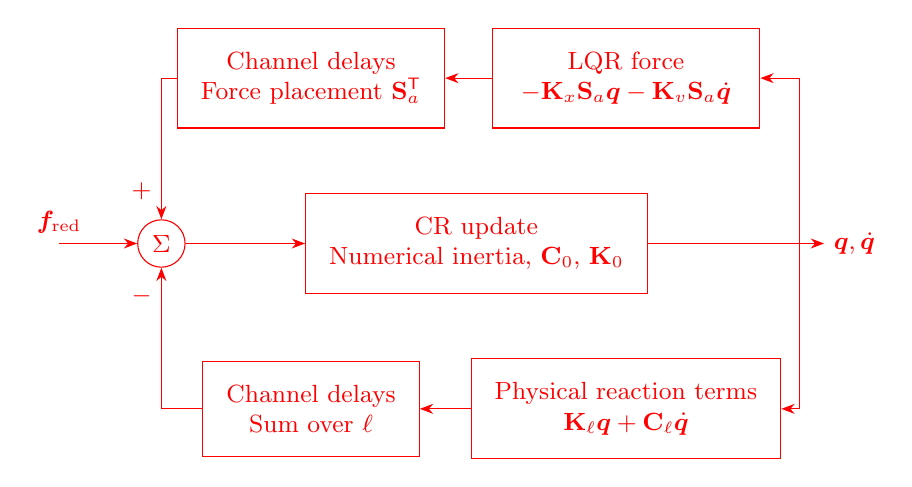
\begin{tikzpicture}[>=Stealth, every node/.style={font=\fontsize{9}{11}\selectfont}, draw=red, text=red,
block/.style={draw=red,rectangle,align=center,minimum height=12mm,inner sep=3mm}]
\node[draw=red,circle,inner sep=1mm] (sum) at (-4,0) {$\Sigma$};
\node[block,minimum width=40mm] (cr) at (0,0) {CR update\\Numerical inertia, $\mathbf C_0$, $\mathbf K_0$};
\node (state) at (4.8,0) {$\bm q,\dot{\bm q}$};
\draw[->,red] (-5.3,0) node[above] {$\bm f_{\mathrm{red}}$} -- (sum);
\draw[->,red] (sum) -- (cr);
\draw[->,red] (cr) -- (state);
\node[block,minimum width=34mm] (lqr) at (1.9,2.1) {LQR force\\$-\mathbf K_x\mathbf S_a\bm q-\mathbf K_v\mathbf S_a\dot{\bm q}$};
\node[block] (ldelay) at (-2.1,2.1) {Channel delays\\Force placement $\mathbf S_a^{\mathsf T}$};
\draw[->,red] (4.1,0) |- (lqr.east);
\draw[->,red] (lqr) -- (ldelay);
\draw[->,red] (ldelay.west) -| node[pos=.9,left] {$+$} (sum.north);
\node[block,minimum width=34mm] (reaction) at (1.9,-2.1) {Physical reaction terms\\$\mathbf K_\ell\bm q+\mathbf C_\ell\dot{\bm q}$};
\node[block] (rdelay) at (-2.1,-2.1) {Channel delays\\Sum over $\ell$};
\draw[->,red] (4.1,0) |- (reaction.east);
\draw[->,red] (reaction) -- (rdelay);
\draw[->,red] (rdelay.west) -| node[pos=.9,left] {$-$} (sum.south);
\end{tikzpicture}

	\caption{\rev{Signal paths of the virtual RTHS with delayed restoring-force and LQR feedback.}}
	\label{fig:rths-loop}
\end{figure}

The retained coordinates of the physical substructure are the only coordinates that the transfer system imposes, and each of them is driven by one actuator. The condensed coordinates are neither commanded nor measured, and their response is reconstructed from the recovery relation of the condensation. The two condensation methods reconstruct this response in different ways.

The reconstructed response follows from Eqs. \eqref{eq:guyan-coordinate-relation} and \eqref{eq:cb-internal-recovery} as

% Removed negative display spacing to prevent equation/text overlap.
\begin{subequations}
	\label{eq:delay-recovery}
	\begin{align}
		\bm{u}_{\mathrm{c}}^{\mathrm{rec}}(t)&=\bm{\Psi}_{\mathrm{G}}\hat{\bm{u}}_{\mathrm{r}}(t),
		\label{eq:guyan-delay-recovery}\\
		\bm{u}_{\mathrm{c}}^{\mathrm{rec}}(t)&=\bm{\Psi}_{\mathrm{G}}\hat{\bm{u}}_{\mathrm{r}}(t)
		+\bm{\Phi}_{d}\bm{\eta}(t),
		\label{eq:cb-delay-recovery}
	\end{align}
\end{subequations}
% Removed negative display spacing to prevent equation/text overlap.

\rev{for Guyan and Craig--Bampton condensation, respectively. The Guyan reconstruction depends on the delayed retained coordinates. The Craig--Bampton modal coordinates \(\bm\eta\) evolve numerically and couple to the delayed retained coordinates through the reduced equations. They do not pass directly through an actuator channel.}

The formulation is developed for a virtual RTHS, in which \(\bm{\eta}\) of the physical substructure is a state of the simulated specimen model.

\subsection{Discrete-time closed-loop pole criterion with LQR control}
\label{sec:pole-criterion}

The assembled reduced model of Eq. \eqref{eq:assembled-reduced} is taken as the starting point. The actuator delay affects only the terms acting on the coordinates imposed by the transfer system, and each channel carries its own delay. The assembled damping and stiffness matrices are therefore split channel by channel, and the equation of motion of the assembled reduced system is

% Removed negative display spacing to prevent equation/text overlap.
\begin{equation}
	\mathbf{M}_{\mathrm{red}}\ddot{\bm{q}}(t)+\mathbf{C}_{0}\dot{\bm{q}}(t)+\mathbf{K}_{0}\bm{q}(t)
	+\sum_{\ell=1}^{n_{\mathrm{a}}}
	\left[
	\mathbf{C}_{\ell}\dot{\bm{q}}(t-\tau_{\ell})
	+\mathbf{K}_{\ell}\bm{q}(t-\tau_{\ell})
	\right]
	=\bm{f}_{\mathrm{red}}(t),
	\label{eq:delayed-eom}
\end{equation}
% Removed negative display spacing to prevent equation/text overlap.

\noindent where \(\bm{q}(t)\) collects the \(n_{q}\) generalized coordinates of the assembled reduced model, \(\mathbf{C}_{\ell}\) and \(\mathbf{K}_{\ell}\) are of the same size as \(\mathbf{C}_{\mathrm{red}}\) and \(\mathbf{K}_{\mathrm{red}}\) and retain only the columns of the reduced physical substructure that act on the coordinate driven by the \(\ell\)th actuator, the remaining columns being zero, and \(\mathbf{C}_{0}=\mathbf{C}_{\mathrm{red}}-\sum_{\ell}\mathbf{C}_{\ell}\) and \(\mathbf{K}_{0}=\mathbf{K}_{\mathrm{red}}-\sum_{\ell}\mathbf{K}_{\ell}\) contain the remaining terms. This split makes the difference described in Section \ref{sec:multiple-delay} explicit. The reduced physical substructure of the Guyan model retains the actuated coordinates alone, and every one of its columns is therefore delayed. The Craig--Bampton model also carries fixed-interface modal coordinates driven by no actuator, and the columns associated with them remain in \(\mathbf{C}_{0}\) and \(\mathbf{K}_{0}\) without delay.

The force returned to the loop by the physical substructure is its elastic and damping reaction to the motion imposed by the transfer system. Each actuated channel therefore enters Eq. \eqref{eq:delayed-eom} with its own delay as a scalar factor, and the delays remain independent of each other. The inertia of the physical substructure is advanced numerically within the assembled state, and the assembled mass matrix carries no delay factor. A term \(\mathbf{M}_{\ell}\ddot{\bm{q}}(t-\tau_{\ell})\) would be added to Eq. \eqref{eq:delayed-eom} once the returned force contained the inertia produced by the delayed motion.

The assembled system of Eq. \eqref{eq:delayed-eom} is advanced with the CR integration algorithm \rev{\cite{ChenCR2008}}, and the sampling period equals the integration time step. A quantity written with the argument \(z\) denotes the \(z\) transform of the corresponding time-domain quantity in the following. The displacement and velocity recursions of the algorithm share one matrix coefficient. Eliminating the acceleration between them and taking the \(z\) transform relates the velocity and the acceleration to the displacement by

% Removed negative display spacing to prevent equation/text overlap.
\begin{equation}
	\begin{gathered}
		\dot{\bm{q}}(z)=\frac{z-1}{z\Delta t}\bm{q}(z),\\
		\mathbf{M}_{\mathrm{red}}\ddot{\bm{q}}(z)=
		\left(\mathbf{M}_{\mathrm{red}}
		+\tfrac{1}{2}\Delta t\,\mathbf{C}_{\mathrm{red}}
		+\tfrac{1}{4}\Delta t^{2}\mathbf{K}_{\mathrm{red}}\right)
		\frac{(z-1)^{2}}{z\Delta t^{2}}\bm{q}(z),
	\end{gathered}
	\label{eq:z-derivatives}
\end{equation}
% Removed negative display spacing to prevent equation/text overlap.

\noindent where the bracket is the mass term of the CR algorithm, formed from the assembled matrices before the channel split of Eq. \eqref{eq:delayed-eom}, since that split describes the signal path of the interface restoring force rather than the time integration. A delay of \(n_{\ell}\) steps becomes the scalar factor \(z^{-n_{\ell}}\). The delayed terms are taken from the stored response history, and the recursion therefore remains explicit in them.

\rev{An LQR supplies an additional force at the actuated coordinates. Its design model is obtained by static condensation of the assembled model onto those coordinates, using their displacements and velocities as states and the applied forces as inputs. The quadratic state and input weights \(\mathbf Q\) and \(\mathbf R\) define the feedback law}

% Removed negative display spacing to prevent equation/text overlap.
\begin{equation}
	\bm{f}_{\mathrm{L}}(t)=
	-\mathbf{K}_{x}\mathbf{S}_{\mathrm{a}}\bm{q}(t)
	-\mathbf{K}_{v}\mathbf{S}_{\mathrm{a}}\dot{\bm{q}}(t),
	\label{eq:lqr-law}
\end{equation}
% Removed negative display spacing to prevent equation/text overlap.

\noindent where \(\mathbf{S}_{\mathrm{a}}\) is the Boolean matrix of size \(n_{\mathrm{a}}\times n_{q}\) that extracts the actuated coordinates from \(\bm{q}\), and \(\mathbf{K}_{x}\) and \(\mathbf{K}_{v}\) are the \(n_{\mathrm{a}}\times n_{\mathrm{a}}\) displacement and velocity parts of the gain.

\rev{The regulator uses the numerical states \(\mathbf S_{\mathrm a}\bm q\) and \(\mathbf S_{\mathrm a}\dot{\bm q}\). Its applied force is
\(\bm f_{\mathrm{L,applied}}(z)=\mathbf S_{\mathrm a}^{\mathsf T}\mathbf H_{\mathrm a}(z)\bm f_{\mathrm L}(z)\),
which enters the right-hand force sum of Eq. \eqref{eq:delayed-eom}. Here \(\mathbf H_{\mathrm a}\) is diagonal with entries \(z^{-n_\ell}\). The law is an output feedback on the assembled model. Equal \(\mathbf Q\) and \(\mathbf R\) yield model-dependent gains, so the resulting domains compare each model together with its regulator.}

% Removed negative display spacing to prevent equation/text overlap.
\begin{equation}
	\begin{aligned}
		\mathbf{Z}(z)={}&
		\frac{(z-1)^{2}}{z\Delta t^{2}}
		\left(\mathbf{M}_{\mathrm{red}}
		+\tfrac{1}{2}\Delta t\,\mathbf{C}_{\mathrm{red}}
		+\tfrac{1}{4}\Delta t^{2}\mathbf{K}_{\mathrm{red}}\right)
		+\frac{z-1}{z\Delta t}\mathbf{C}_{0}+\mathbf{K}_{0}\\
		&+\sum_{\ell=1}^{n_{\mathrm{a}}}z^{-n_{\ell}}
		\left[
		\frac{z-1}{z\Delta t}\mathbf{C}_{\ell}+\mathbf{K}_{\ell}
		\right]
		+\mathbf{S}_{\mathrm{a}}^{\mathsf{T}}\mathbf{H}_{\mathrm{a}}(z)
		\left[
		\mathbf{K}_{x}+\frac{z-1}{z\Delta t}\mathbf{K}_{v}
		\right]\mathbf{S}_{\mathrm{a}},
	\end{aligned}
	\label{eq:z-matrix}
\end{equation}
% Removed negative display spacing to prevent equation/text overlap.

\noindent where \(\mathbf{H}_{\mathrm{a}}(z)\) is the diagonal matrix whose \(\ell\)th entry is the delay factor \(z^{-n_{\ell}}\) of the \(\ell\)th channel. The poles of the closed-loop system are the roots of

% Removed negative display spacing to prevent equation/text overlap.
\begin{equation}
	\det\mathbf{Z}(z)=0.
	\label{eq:characteristic-equation}
\end{equation}
% Removed negative display spacing to prevent equation/text overlap.

The negative powers of \(z\) in Eq. \eqref{eq:z-matrix} are cleared by multiplying Eq. \eqref{eq:characteristic-equation} by a sufficient power of \(z\), and the roots introduced at the origin by this operation are discarded.

The continuous and the discrete planes are related by \(z=\mathrm{e}^{s\Delta t}\), and the left half of the \(s\) plane therefore maps onto the interior of the unit circle of the \(z\) plane. The largest modulus among the roots of Eq. \eqref{eq:characteristic-equation} is written as \(\rho_{\mathrm{cl}}\). The system is stable when \(\rho_{\mathrm{cl}}<1\), unstable when \(\rho_{\mathrm{cl}}>1\), and on the stability boundary when \(\rho_{\mathrm{cl}}=1\).

For a given condensed model, \(\rho_{\mathrm{cl}}\) depends on the delay of each actuator through the factors \(z^{-n_{\ell}}\). The stability domain is obtained by evaluating \(\rho_{\mathrm{cl}}\) over combinations of the integer delays \(n_{\ell}\) and by locating the contour on which \(\rho_{\mathrm{cl}}\) equals unity. The delays are expressed in multiples of the sampling period, and the resulting domain gives the combinations of actuator delays for which the RTHS system remains stable.




\section{Benchmark structure and analysis setup} \label{sec4}

\rev{The benchmark uses two coordinate selections associated with the designated substructure divisions. The frame properties, implemented accuracy models, excitations and evaluation indices are specified below.}

\subsection{Benchmark structure and finite element idealization}
\label{sec:benchmark}

The reference structure is a simplified planar model built from the \rev{geometry} of the multi-axial RTHS benchmark frame of Condori Uribe et al. \cite{Condori2023}. The three bays are 762 mm wide and the three storeys are 635 mm high. \rev{The model uses the member properties specified below, with A992 Gr.50 steel for the columns and A36 steel for the beams.} \rev{The geometry is shown in Fig. \ref{fig:benchmark-geometry}, and Table \ref{tab:materials} lists the material properties used in the model.}

\begin{figure}[htbp]
	\centering
	% Selected option: Figure 3-C. Compare with TU thesis Fig. 2-3 (PDF p.28).
	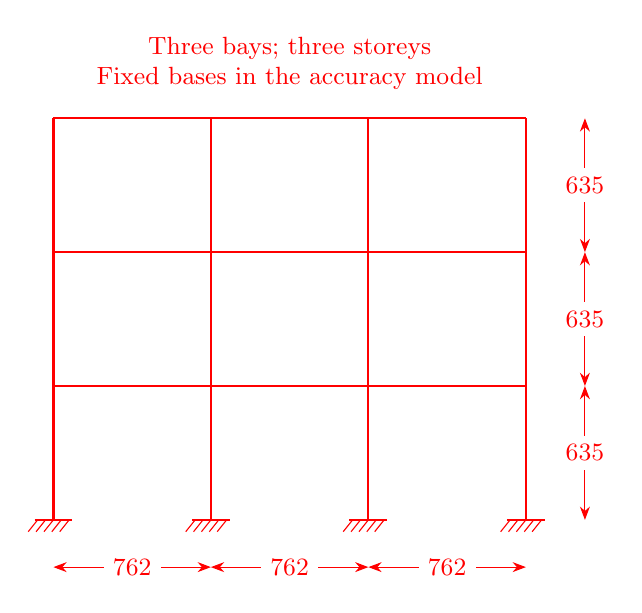
\begin{tikzpicture}[>=Stealth,every node/.style={font=\fontsize{9}{11}\selectfont,text=red}]
\begin{scope}[shift={(0,0)},scale=1]
\draw[red,line width=.8pt] (0,0)--(0,5.1);
\draw[red,line width=.7pt] (-0.24,0)--(0.24,0);
\draw[red,line width=.4pt] (-0.2,0)--(-0.32,-.15);
\draw[red,line width=.4pt] (-0.1,0)--(-0.22,-.15);
\draw[red,line width=.4pt] (0,0)--(-0.12,-.15);
\draw[red,line width=.4pt] (0.1,0)--(-0.01999999999999999,-.15);
\draw[red,line width=.4pt] (0.2,0)--(0.08000000000000002,-.15);
\draw[red,line width=.8pt] (2,0)--(2,5.1);
\draw[red,line width=.7pt] (1.76,0)--(2.24,0);
\draw[red,line width=.4pt] (1.8,0)--(1.6800000000000002,-.15);
\draw[red,line width=.4pt] (1.9,0)--(1.7799999999999998,-.15);
\draw[red,line width=.4pt] (2,0)--(1.88,-.15);
\draw[red,line width=.4pt] (2.1,0)--(1.98,-.15);
\draw[red,line width=.4pt] (2.2,0)--(2.08,-.15);
\draw[red,line width=.8pt] (4,0)--(4,5.1);
\draw[red,line width=.7pt] (3.76,0)--(4.24,0);
\draw[red,line width=.4pt] (3.8,0)--(3.6799999999999997,-.15);
\draw[red,line width=.4pt] (3.9,0)--(3.78,-.15);
\draw[red,line width=.4pt] (4,0)--(3.88,-.15);
\draw[red,line width=.4pt] (4.1,0)--(3.9799999999999995,-.15);
\draw[red,line width=.4pt] (4.2,0)--(4.08,-.15);
\draw[red,line width=.8pt] (6,0)--(6,5.1);
\draw[red,line width=.7pt] (5.76,0)--(6.24,0);
\draw[red,line width=.4pt] (5.8,0)--(5.68,-.15);
\draw[red,line width=.4pt] (5.9,0)--(5.78,-.15);
\draw[red,line width=.4pt] (6,0)--(5.88,-.15);
\draw[red,line width=.4pt] (6.1,0)--(5.9799999999999995,-.15);
\draw[red,line width=.4pt] (6.2,0)--(6.08,-.15);
\draw[red,line width=.8pt] (0,1.7)--(6,1.7);
\draw[red,line width=.8pt] (0,3.4)--(6,3.4);
\draw[red,line width=.8pt] (0,5.1)--(6,5.1);
\end{scope}\draw[red,<->] (0,-.6)--(2,-.6) node[midway,fill=white] {762};
\draw[red,<->] (2,-.6)--(4,-.6) node[midway,fill=white] {762};
\draw[red,<->] (4,-.6)--(6,-.6) node[midway,fill=white] {762};
\draw[red,<->] (6.75,0.0)--(6.75,1.7) node[midway,fill=white] {635};
\draw[red,<->] (6.75,1.7)--(6.75,3.4) node[midway,fill=white] {635};
\draw[red,<->] (6.75,3.4)--(6.75,5.1) node[midway,fill=white] {635};
\node[red,align=center] at (3,5.8) {Three bays; three storeys\\Fixed bases in the accuracy model};
\end{tikzpicture}
	\caption{\rev{Geometry of the three-storey frame used in the accuracy benchmark. Dimensions are in mm.}}
	\label{fig:benchmark-geometry}
\end{figure}

\begin{table}[htbp]
	\centering
	\caption{Material properties of the benchmark frame.}
	\label{tab:materials}
	\begin{tabular}{lccccc}
		\toprule
		Steel grade & \(f_{\mathrm{y}}\) (MPa) & \(f_{\mathrm{u}}\) (MPa) & \(E\) (GPa) & \(\nu\) & \(\rho\) (kg/m\(^{3}\))\\
		\midrule
		A36 (beams)      & 250 & 400--550 & \rev{206} & 0.3 & 7850\\
		A992 Gr.50 (columns) & 345 & 450--550 & \rev{206} & 0.3 & 7850\\
		\bottomrule
	\end{tabular}
\end{table}

In the finite element idealization, each node of the frame carries two in-plane translations and one rotation about the out-of-plane axis. The frame responds mainly in the horizontal direction under a base excitation. The axial deformation of the members is therefore neglected, the vertical displacement is taken as zero, and the horizontal displacement is assumed identical for all nodes of a storey. The idealized model of Fig. \ref{fig:dof-idealization} has fifteen DOFs, which are one horizontal displacement per storey and one rotation at each of the four nodes of each storey. Among them, \(\psi_{1}\), \(\psi_{6}\) and \(\psi_{11}\) are the horizontal displacements of the first, second and third storey, and the remaining coordinates are the nodal rotations of the corresponding storey.

\begin{figure}[htbp]
	\centering
	% Selected option: Figure 4-D.
	% Panel (a): TU thesis Fig. 2-4 (PDF p.29); panel (b): Fig. 2-5 (PDF p.30).
	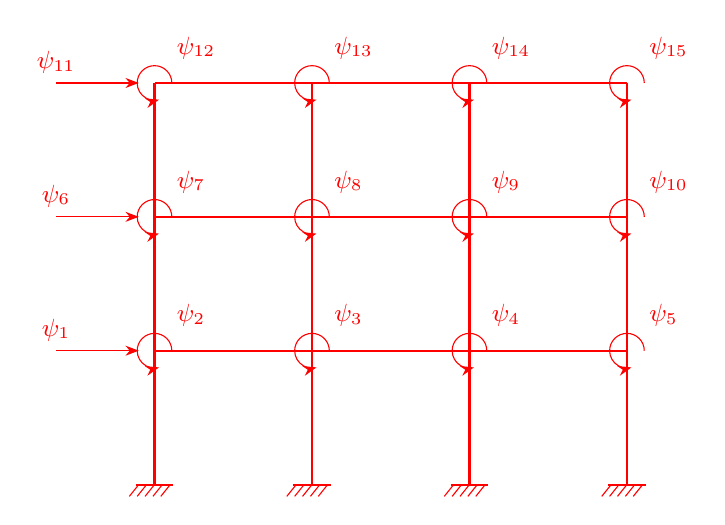
\begin{tikzpicture}[>=Stealth,every node/.style={font=\fontsize{9}{11}\selectfont,text=red}]
\begin{scope}[shift={(0,0)},scale=1]
\draw[red,line width=.8pt] (0,0)--(0,5.1);
\draw[red,line width=.7pt] (-0.24,0)--(0.24,0);
\draw[red,line width=.4pt] (-0.2,0)--(-0.32,-.15);
\draw[red,line width=.4pt] (-0.1,0)--(-0.22,-.15);
\draw[red,line width=.4pt] (0,0)--(-0.12,-.15);
\draw[red,line width=.4pt] (0.1,0)--(-0.01999999999999999,-.15);
\draw[red,line width=.4pt] (0.2,0)--(0.08000000000000002,-.15);
\draw[red,line width=.8pt] (2,0)--(2,5.1);
\draw[red,line width=.7pt] (1.76,0)--(2.24,0);
\draw[red,line width=.4pt] (1.8,0)--(1.6800000000000002,-.15);
\draw[red,line width=.4pt] (1.9,0)--(1.7799999999999998,-.15);
\draw[red,line width=.4pt] (2,0)--(1.88,-.15);
\draw[red,line width=.4pt] (2.1,0)--(1.98,-.15);
\draw[red,line width=.4pt] (2.2,0)--(2.08,-.15);
\draw[red,line width=.8pt] (4,0)--(4,5.1);
\draw[red,line width=.7pt] (3.76,0)--(4.24,0);
\draw[red,line width=.4pt] (3.8,0)--(3.6799999999999997,-.15);
\draw[red,line width=.4pt] (3.9,0)--(3.78,-.15);
\draw[red,line width=.4pt] (4,0)--(3.88,-.15);
\draw[red,line width=.4pt] (4.1,0)--(3.9799999999999995,-.15);
\draw[red,line width=.4pt] (4.2,0)--(4.08,-.15);
\draw[red,line width=.8pt] (6,0)--(6,5.1);
\draw[red,line width=.7pt] (5.76,0)--(6.24,0);
\draw[red,line width=.4pt] (5.8,0)--(5.68,-.15);
\draw[red,line width=.4pt] (5.9,0)--(5.78,-.15);
\draw[red,line width=.4pt] (6,0)--(5.88,-.15);
\draw[red,line width=.4pt] (6.1,0)--(5.9799999999999995,-.15);
\draw[red,line width=.4pt] (6.2,0)--(6.08,-.15);
\draw[red,line width=.8pt] (0,1.7)--(6,1.7);
\draw[red,->] (0.22,1.7) arc (0:285:.22);
\node[above right,text=red] at (0.16,1.88) {$\psi_{2}$};
\draw[red,->] (2.22,1.7) arc (0:285:.22);
\node[above right,text=red] at (2.16,1.88) {$\psi_{3}$};
\draw[red,->] (4.22,1.7) arc (0:285:.22);
\node[above right,text=red] at (4.16,1.88) {$\psi_{4}$};
\draw[red,->] (6.22,1.7) arc (0:285:.22);
\node[above right,text=red] at (6.16,1.88) {$\psi_{5}$};
\draw[red,->] (-1.25,1.7)--(-.2,1.7) node[pos=0,above] {$\psi_{1}$};
\draw[red,line width=.8pt] (0,3.4)--(6,3.4);
\draw[red,->] (0.22,3.4) arc (0:285:.22);
\node[above right,text=red] at (0.16,3.58) {$\psi_{7}$};
\draw[red,->] (2.22,3.4) arc (0:285:.22);
\node[above right,text=red] at (2.16,3.58) {$\psi_{8}$};
\draw[red,->] (4.22,3.4) arc (0:285:.22);
\node[above right,text=red] at (4.16,3.58) {$\psi_{9}$};
\draw[red,->] (6.22,3.4) arc (0:285:.22);
\node[above right,text=red] at (6.16,3.58) {$\psi_{10}$};
\draw[red,->] (-1.25,3.4)--(-.2,3.4) node[pos=0,above] {$\psi_{6}$};
\draw[red,line width=.8pt] (0,5.1)--(6,5.1);
\draw[red,->] (0.22,5.1) arc (0:285:.22);
\node[above right,text=red] at (0.16,5.279999999999999) {$\psi_{12}$};
\draw[red,->] (2.22,5.1) arc (0:285:.22);
\node[above right,text=red] at (2.16,5.279999999999999) {$\psi_{13}$};
\draw[red,->] (4.22,5.1) arc (0:285:.22);
\node[above right,text=red] at (4.16,5.279999999999999) {$\psi_{14}$};
\draw[red,->] (6.22,5.1) arc (0:285:.22);
\node[above right,text=red] at (6.16,5.279999999999999) {$\psi_{15}$};
\draw[red,->] (-1.25,5.1)--(-.2,5.1) node[pos=0,above] {$\psi_{11}$};
\end{scope}
\end{tikzpicture}
	\caption{\rev{Coordinate order of the fifteen-DOF model: three storey translations and twelve nodal rotations.}}
	\label{fig:dof-idealization}
\end{figure}

\rev{The accuracy benchmark fixes the translations and rotations at all four column bases. It uses \(A_{\mathrm c}=1.670\,\mathrm{in}^{2}\), \(A_{\mathrm b}=0.947\,\mathrm{in}^{2}\), \(I_{\mathrm c}=2.520\,\mathrm{in}^{4}\) and \(I_{\mathrm b}=0.6132\,\mathrm{in}^{4}\). The diagonal mass matrix repeats one five-entry block per storey: a translational mass of 6164.8306 kg followed by rotational inertias of 51.0878, 67.8872, 67.8872 and 51.0878 kg\,m\(^{2}\). These values use an effective mass density of \(190\times7850\) kg/m\(^{3}\) in the lumped-mass construction. Rayleigh damping, \(\mathbf C=a_0\mathbf M+a_1\mathbf K\), gives 5\% damping at the first two modes, with \(a_0=1.3184625\) s\(^{-1}\) and \(a_1=0.0013223424\) s. The same full-order damping matrix is reduced with each model. The first five frequencies are 2.7074, 9.3284, 18.4427, 22.6736 and 24.2277 Hz, accounting for 98.0608\% of the horizontal effective modal mass. The full matrices and coordinate order are supplied in the supplementary data.}

\subsection{Substructure division and selection of retained DOFs}
\label{sec:division}

The position of the boundary between the physical and the numerical substructures affects both the dynamic response and the accuracy of the condensation. Two divisions are compared and both are shown in Fig. \ref{fig:division}. In each of them the outer bay of the frame is implemented as the physical substructure and the remaining part forms the numerical substructure. The outer bay is selected because a division at an inner bay would split the numerical substructure into two separate parts.

In division I the physical substructure covers the first two storeys of the outer bay together with the connected beams and columns. The lower storeys carry the largest storey shear of the first two modes, and the interface is close to the actuator locations, which shortens the loading path. 

In division II the physical substructure covers all three storeys of the outer bay. 

Three requirements govern the selection of the retained coordinates. The coordinates carrying the dominant response remain explicit, the condensed response is recoverable through the relations of Section \ref{sec2}, and the reduction is large enough to be of practical use. The horizontal storey displacements govern the global response of a frame under a base excitation and carry most of the energy of the low-order modes. \rev{The retained rotations preserve selected bending coordinates; the remaining rotations are recovered through the reduction basis.}

\rev{Both divisions assign two actuator channels. They act at \(\psi_1,\psi_6\) in division I and at \(\psi_1,\psi_{11}\) in division II. The accuracy comparison uses the corresponding whole-structure coordinate selections in Table \ref{tab:dof-sets}. Division II condenses the middle-storey translation \(\psi_6\), whereas division I retains all three storey translations. Both selections retain the rotations \(\psi_4,\psi_9,\psi_{14}\).}

\rev{For the accuracy calculations, reduction is applied once to the assembled fifteen-DOF matrices. Each reduced response is expanded to the original coordinate order, giving one recovered value per coordinate.}

\begin{figure}[htbp]
	\centering
	% Selected option: Figure 5-D.
	% Panel (a): TU thesis Fig. 3-1; panel (b): Fig. 3-2; both on PDF p.37.
	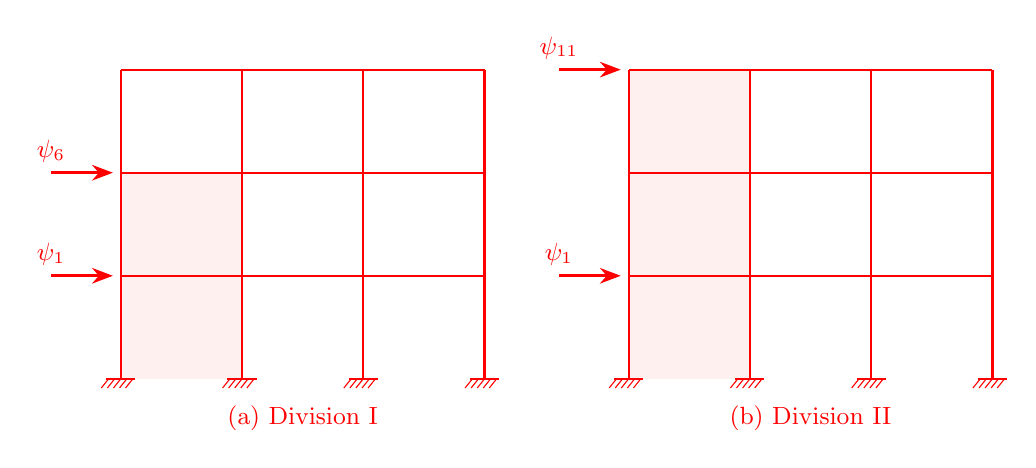
\begin{tikzpicture}[>=Stealth,every node/.style={font=\fontsize{9}{11}\selectfont,text=red}]
\begin{scope}[shift={(0,0)},scale=0.77]
\fill[red,opacity=.06] (0,0) rectangle (2,3.4);
\draw[red,line width=.8pt] (0,0)--(0,5.1);
\draw[red,line width=.7pt] (-0.24,0)--(0.24,0);
\draw[red,line width=.4pt] (-0.2,0)--(-0.32,-.15);
\draw[red,line width=.4pt] (-0.1,0)--(-0.22,-.15);
\draw[red,line width=.4pt] (0,0)--(-0.12,-.15);
\draw[red,line width=.4pt] (0.1,0)--(-0.01999999999999999,-.15);
\draw[red,line width=.4pt] (0.2,0)--(0.08000000000000002,-.15);
\draw[red,line width=.8pt] (2,0)--(2,5.1);
\draw[red,line width=.7pt] (1.76,0)--(2.24,0);
\draw[red,line width=.4pt] (1.8,0)--(1.6800000000000002,-.15);
\draw[red,line width=.4pt] (1.9,0)--(1.7799999999999998,-.15);
\draw[red,line width=.4pt] (2,0)--(1.88,-.15);
\draw[red,line width=.4pt] (2.1,0)--(1.98,-.15);
\draw[red,line width=.4pt] (2.2,0)--(2.08,-.15);
\draw[red,line width=.8pt] (4,0)--(4,5.1);
\draw[red,line width=.7pt] (3.76,0)--(4.24,0);
\draw[red,line width=.4pt] (3.8,0)--(3.6799999999999997,-.15);
\draw[red,line width=.4pt] (3.9,0)--(3.78,-.15);
\draw[red,line width=.4pt] (4,0)--(3.88,-.15);
\draw[red,line width=.4pt] (4.1,0)--(3.9799999999999995,-.15);
\draw[red,line width=.4pt] (4.2,0)--(4.08,-.15);
\draw[red,line width=.8pt] (6,0)--(6,5.1);
\draw[red,line width=.7pt] (5.76,0)--(6.24,0);
\draw[red,line width=.4pt] (5.8,0)--(5.68,-.15);
\draw[red,line width=.4pt] (5.9,0)--(5.78,-.15);
\draw[red,line width=.4pt] (6,0)--(5.88,-.15);
\draw[red,line width=.4pt] (6.1,0)--(5.9799999999999995,-.15);
\draw[red,line width=.4pt] (6.2,0)--(6.08,-.15);
\draw[red,line width=.8pt] (0,1.7)--(6,1.7);
\draw[red,->,line width=1pt] (-1.15,1.7)--(-.13,1.7) node[pos=0,above] {$\psi_{1}$};
\draw[red,line width=.8pt] (0,3.4)--(6,3.4);
\draw[red,->,line width=1pt] (-1.15,3.4)--(-.13,3.4) node[pos=0,above] {$\psi_{6}$};
\draw[red,line width=.8pt] (0,5.1)--(6,5.1);
\node[text=red] at (3,-.65) {(a) Division I};
\end{scope}
\begin{scope}[shift={(6.45,0)},scale=0.77]
\fill[red,opacity=.06] (0,0) rectangle (2,5.1);
\draw[red,line width=.8pt] (0,0)--(0,5.1);
\draw[red,line width=.7pt] (-0.24,0)--(0.24,0);
\draw[red,line width=.4pt] (-0.2,0)--(-0.32,-.15);
\draw[red,line width=.4pt] (-0.1,0)--(-0.22,-.15);
\draw[red,line width=.4pt] (0,0)--(-0.12,-.15);
\draw[red,line width=.4pt] (0.1,0)--(-0.01999999999999999,-.15);
\draw[red,line width=.4pt] (0.2,0)--(0.08000000000000002,-.15);
\draw[red,line width=.8pt] (2,0)--(2,5.1);
\draw[red,line width=.7pt] (1.76,0)--(2.24,0);
\draw[red,line width=.4pt] (1.8,0)--(1.6800000000000002,-.15);
\draw[red,line width=.4pt] (1.9,0)--(1.7799999999999998,-.15);
\draw[red,line width=.4pt] (2,0)--(1.88,-.15);
\draw[red,line width=.4pt] (2.1,0)--(1.98,-.15);
\draw[red,line width=.4pt] (2.2,0)--(2.08,-.15);
\draw[red,line width=.8pt] (4,0)--(4,5.1);
\draw[red,line width=.7pt] (3.76,0)--(4.24,0);
\draw[red,line width=.4pt] (3.8,0)--(3.6799999999999997,-.15);
\draw[red,line width=.4pt] (3.9,0)--(3.78,-.15);
\draw[red,line width=.4pt] (4,0)--(3.88,-.15);
\draw[red,line width=.4pt] (4.1,0)--(3.9799999999999995,-.15);
\draw[red,line width=.4pt] (4.2,0)--(4.08,-.15);
\draw[red,line width=.8pt] (6,0)--(6,5.1);
\draw[red,line width=.7pt] (5.76,0)--(6.24,0);
\draw[red,line width=.4pt] (5.8,0)--(5.68,-.15);
\draw[red,line width=.4pt] (5.9,0)--(5.78,-.15);
\draw[red,line width=.4pt] (6,0)--(5.88,-.15);
\draw[red,line width=.4pt] (6.1,0)--(5.9799999999999995,-.15);
\draw[red,line width=.4pt] (6.2,0)--(6.08,-.15);
\draw[red,line width=.8pt] (0,1.7)--(6,1.7);
\draw[red,->,line width=1pt] (-1.15,1.7)--(-.13,1.7) node[pos=0,above] {$\psi_{1}$};
\draw[red,line width=.8pt] (0,3.4)--(6,3.4);
\draw[red,line width=.8pt] (0,5.1)--(6,5.1);
\draw[red,->,line width=1pt] (-1.15,5.1)--(-.13,5.1) node[pos=0,above] {$\psi_{11}$};
\node[text=red] at (3,-.65) {(b) Division II};
\end{scope}
\end{tikzpicture}
\caption{\rev{Substructure divisions and actuator assignments. Shading marks the designated physical region; arrows mark the two actuator channels.}}


\label{fig:division}
\end{figure}

\begin{table}[htbp]
\centering
\caption{\rev{Whole-structure coordinate selections used in the accuracy calculations.}}
\label{tab:dof-sets}
{\color{red}
\begin{tabular}{lllcc}
\toprule
Division & Retained coordinate indices & Actuated indices & Static order & CB order\\
\midrule
I & 1, 6, 11, 4, 9, 14 & 1, 6 & 6 & 9\\
II & 1, 11, 4, 9, 14 & 1, 11 & 5 & 8\\
\bottomrule
\end{tabular}}
\end{table}

\rev{The Craig--Bampton models use the three lowest fixed-interface modes of the global condensed set and the congruent projection of Eq. \eqref{eq:general-projection}. The static implementation used for the reported accuracy results retains the first block row after imposing \(\bm u_{\mathrm c}=\bm\Psi_{\mathrm G}\bm u_{\mathrm r}\):
\(\mathbf M_{\mathrm G}=\mathbf M_{\mathrm{rr}}+\mathbf M_{\mathrm{rc}}\bm\Psi_{\mathrm G}\),
\(\mathbf C_{\mathrm G}=\mathbf C_{\mathrm{rr}}+\mathbf C_{\mathrm{rc}}\bm\Psi_{\mathrm G}\), and
\(\mathbf K_{\mathrm G}=\mathbf K_{\mathrm{rr}}+\mathbf K_{\mathrm{rc}}\bm\Psi_{\mathrm G}\), with
\(\bm f_{\mathrm G}=\mathbf T_{\mathrm G}^{\mathsf T}\bm f\).
It is labelled Guyan in the tables and response plots. This retained-equation implementation differs from the congruent Guyan projection of Section \ref{sec21}; the accuracy results refer to the stated implementation.}

\subsection{Simulation setup and evaluation indices}
\label{sec:setup}

\rev{The full-order and reduced equations are integrated in Simulink using fixed-step fourth-order Runge--Kutta integration, with \(\Delta t=1/1024\) s, a 40 s duration and zero initial conditions. Accuracy calculations set \(\bm f_{\mathrm L}=\bm0\) and all delays to zero. The full seismic force is projected into each reduced system, and storey displacements are recovered through its transformation matrix.}

\rev{The earthquake input is the El Centro 1940 north--south acceleration record in m/s\(^{2}\), multiplied by 0.40 and linearly interpolated during integration. The chirp acceleration is \(a_{\mathrm g}(t)=\sin[2\pi(0.1)t+\pi(0.2475)t^2]\) m/s\(^{2}\) for \(0\leq t\leq40\) s, with unit amplitude and zero initial phase. Its instantaneous frequency, \(f(t)=0.1+0.2475t\), crosses the first two modes.}

\rev{The stability formulation uses the same sampling period and the two channel assignments above, with independent constant delays. The regulator uses diagonal weights: \(10^6\) for each displacement, \(10^4\) for each velocity and \(10^{-2}\) for each force input. Figure \ref{fig:stability-domain} retains the boundary data from the original analysis; its generating substructure matrices and regulator gains are not available as a complete reproducible set. The current whole-structure accuracy calculations therefore supply Tables \ref{tab:modal}--\ref{tab:energy} independently of those boundary data.}

Three indices are adopted for the accuracy of the condensed models. The first is the relative error of the natural frequencies, \(e_{f,i}=|f_{i}^{\mathrm{full}}-f_{i}^{\mathrm{red}}|/f_{i}^{\mathrm{full}}\times100\%\), where \(f_{i}^{\mathrm{full}}\) and \(f_{i}^{\mathrm{red}}\) are the \(i\)th natural frequency of the full-order and of the condensed model. The second is the modal assurance criterion,

% Removed negative display spacing to prevent equation/text overlap.
\begin{equation}
	\mathrm{MAC}_{i}=
	\frac{\left[\left(\bm{\varphi}_{i}^{\mathrm{full}}\right)^{\mathsf{T}}
		\bm{\varphi}_{i}^{\mathrm{red}}\right]^{2}}
	{\left\|\bm{\varphi}_{i}^{\mathrm{full}}\right\|^{2}
		\left\|\bm{\varphi}_{i}^{\mathrm{red}}\right\|^{2}},
	\label{eq:mac}
\end{equation}
% Removed negative display spacing to prevent equation/text overlap.

\noindent where \(\bm{\varphi}_{i}^{\mathrm{red}}\) is the \(i\)th mode shape of the condensed model and \(\bm{\varphi}_{i}^{\mathrm{full}}\) is the \(i\)th mode shape of the full-order model restricted to the retained coordinates, which places the two vectors on the same coordinate set. The retained-coordinate part of the reduced mode shape is taken for the Craig--Bampton models. \rev{The retained translations are expressed in metres and rotations in radians without further scaling. This MAC is specific to that coordinate convention.} The third is the normalized root mean square error of the time histories,

% Removed negative display spacing to prevent equation/text overlap.
\begin{equation}
	\mathrm{NRMSE}=
	\frac{\displaystyle\sqrt{\frac{1}{T_{\mathrm{d}}}\int_{0}^{T_{\mathrm{d}}}
			\left[x^{\mathrm{full}}(t)-x^{\mathrm{red}}(t)\right]^{2}\mathrm{d}t}}
	{\max\left(x^{\mathrm{full}}\right)-\min\left(x^{\mathrm{full}}\right)}
	\times100\%,
	\label{eq:nrmse}
\end{equation}
% Removed negative display spacing to prevent equation/text overlap.

\noindent where \(x^{\mathrm{full}}\) and \(x^{\mathrm{red}}\) are the horizontal storey displacements of the full-order and of the condensed model, and \(T_{\mathrm{d}}\) is the duration of the response. For a frequency band, the numerator is evaluated over the corresponding time interval and divided by the duration of that interval, which places bands of different length on the same root mean square basis. The denominator is the peak-to-peak value of the full-order response over the whole record and is common to every band, and a band of small response amplitude therefore returns a small NRMSE.

\rev{The chirp bands use the frequency limits 0.1, 1.9, 3.5, 5.4, 8.1 and 10 Hz. These limits approximate multiples of the 2.7074 Hz fundamental frequency and are used directly to define the integration intervals through \(t=(f-0.1)/0.2475\). Squared errors are integrated by the trapezoidal rule, with linear interpolation at the band endpoints. The 1.9--3.5 Hz band spans 7.2727--13.7374 s. Each band includes transients generated earlier in the sweep, so the values describe changes across sweep stages.}

\rev{A signed modal-share index describes the change at the actuated coordinates. For mass-normalized modes, the coordinate share is}

% Removed negative display spacing to prevent equation/text overlap.
\begin{equation}
	\begin{gathered}
		\gamma_{i}=
		\frac{\bm{\varphi}_{i}^{\mathsf{T}}\mathbf{M}\bm{\Gamma}}
		{\bm{\varphi}_{i}^{\mathsf{T}}\mathbf{M}\bm{\varphi}_{i}},
		\qquad
		p_{i}=\frac{\gamma_{i}^{2}}{\displaystyle\sum_{k=1}^{m}\gamma_{k}^{2}},\\[2pt]
		E_{j}=\sum_{i=1}^{m}p_{i}\,
		\frac{m_{j}\varphi_{j,i}^{2}}{\displaystyle\sum_{l=1}^{n}m_{l}\varphi_{l,i}^{2}},
	\end{gathered}
	\label{eq:dof-energy}
\end{equation}
% Removed negative display spacing to prevent equation/text overlap.

\noindent where \(\gamma_{i}\) is the modal participation factor of the \(i\)th mode, \(p_{i}\) is the corresponding modal weight, \(E_{j}\) is the modal share of coordinate \(j\), \(\bm{\varphi}_{i}\) is the \(i\)th mode shape and \(\varphi_{j,i}\) is its \(j\)th entry, \(\bm{\Gamma}\) is the influence vector of Eq. \eqref{eq:full-order-eom}, \(m_{j}\) is the diagonal entry of the mass matrix associated with coordinate \(j\), \(n\) is the number of DOFs of the full-order model, and \(m\) is the number of modes considered, taken as \(m=5\) for the frame of Section \ref{sec:benchmark}. \rev{Each reduced mode is expanded by its global transformation, restored to the original fifteen-coordinate order and normalized using \(\bm\varphi_i^{\mathsf T}\mathbf M\bm\varphi_i=1\) with the full-order mass matrix. The first five modes of each model are used, with their own participation weights. The signed index is}

% Removed negative display spacing to prevent equation/text overlap.
\begin{equation}
	\Delta E=\sum_{k=1}^{n_{\mathrm{a}}}
	\frac{E^{\mathrm{red}}(d_{k})-E^{\mathrm{full}}(d_{k})}{E^{\mathrm{full}}(d_{k})}.
	\label{eq:energy-change}
\end{equation}
% Removed negative display spacing to prevent equation/text overlap.

\rev{\noindent where \(d_k\) is an actuated coordinate and \(E^{\mathrm{full}}\) and \(E^{\mathrm{red}}\) are the corresponding modal shares. The index sums their relative changes and retains their signs. It describes a mass-weighted modal distribution; the closed-loop poles determine delay stability.}




\section{Results and discussion} \label{sec5}

\rev{The results compare the modal properties and delay-free responses of the implemented reductions, followed by the reported stability boundaries and the signed modal-share indices.}

\subsection{Modal accuracy}
\label{sec:modal-accuracy}

\rev{Table \ref{tab:modal} compares the two reference modes within the 0.1--10 Hz excitation range, at 2.7074 and 9.3284 Hz. The maximum Craig--Bampton frequency error is 0.284\%. The Guyan errors are 0.648\% and 5.411\% in division I, increasing to 19.040\% and 30.574\% in division II.}

\begin{table}[htbp]
	\centering
	\caption{Relative error of the natural frequencies and MAC values of the condensed models.}
	\label{tab:modal}
	\begin{tabular}{llcccc}
		\toprule
		& & \multicolumn{2}{c}{Frequency error (\%)} & \multicolumn{2}{c}{MAC}\\
		\cmidrule(lr){3-4}\cmidrule(lr){5-6}
		Division & Mode & Guyan & Craig--Bampton & Guyan & Craig--Bampton\\
		\midrule
		I  & 1 & 0.648& 0.003& 1.0000& 1.0000\\
		I  & 2 & 5.411& 0.284& 0.9998& 1.0000\\
		\midrule
		II & 1 & \rev{19.040}& \rev{0.024}& 0.9962& 1.0000\\
		II & 2 & \rev{30.574}& \rev{0.108}& 0.9255& \rev{1.0000}\\
		\bottomrule
	\end{tabular}
\end{table}

\rev{Condensing the middle-storey translation makes the static model more sensitive to the approximation of internal dynamics. The implemented Guyan model shifts both frequencies upward in division II. Craig--Bampton enrichment retains internal vibration patterns and reduces these errors to 0.024\% and 0.108\%.}

\rev{The retained-coordinate MAC remains above 0.92 in every case. In division II, the Guyan second-mode MAC is 0.9255 despite a 30.574\% frequency error. Retained-coordinate correlation alone therefore gives an incomplete measure of dynamic accuracy; it must be considered alongside the frequency and response errors.}

\subsection{Response accuracy under earthquake and chirp excitation}
\label{sec:response-accuracy}

\rev{Figs. \ref{fig:eq-div1} and \ref{fig:eq-div2} compare first- and third-storey displacements under El Centro excitation. The Guyan deviation is modest in division I and more pronounced in division II, while Craig--Bampton follows the reference closely. The recovered middle-storey displacement in division II gives full-record NRMSE values of 10.798\% for Guyan and 0.031\% for Craig--Bampton. These values evaluate the single global recovery of \(\psi_6\) used in the accuracy model.}

\begin{figure}[htbp]
	\centering
	% Calculation-result plot: source/results mapping in figure/results_v2.
	% Compare with TU thesis Fig. 3-6 (PDF p.42) and Fig. 3-8 (PDF p.43).
	\includegraphics[width=0.98\textwidth]{fig06_eq_div1.pdf}
	\caption{Horizontal storey displacement of division I under the El Centro record. (a) First storey. (b) Third storey.}
	\label{fig:eq-div1}
\end{figure}

\begin{figure}[htbp]
	\centering
	% Calculation-result plot: source/results mapping in figure/results_v2.
	% Compare with TU thesis Fig. 3-9 (PDF p.44) and Fig. 3-10 (PDF p.45).
	\includegraphics[width=0.98\textwidth]{fig07_eq_div2.pdf}
	\caption{Horizontal storey displacement of division II under the El Centro record. (a) First storey. (b) Third storey.}
	\label{fig:eq-div2}
\end{figure}

\rev{Figs. \ref{fig:chirp-div1} and \ref{fig:chirp-div2} show the chirp responses. The sweep crosses the reference fundamental frequency at 10.5351 s, and the largest absolute reference displacement occurs near 11.69 s. The 13--14 s insets show the subsequent resonant response.}

\rev{In division I, the Guyan deviation grows again in the 38--38.3 s window, near the second-mode response. In division II, the shifted static-model resonances produce larger amplitude and phase differences. Over that final window, its first- and third-storey peak-to-peak displacements are 46\% and 81\% of the reference values, respectively. Craig--Bampton follows the reference throughout the sweep. For the recovered middle-storey displacement in division II, the full-record NRMSE is 11.749\% for Guyan and 0.034\% for Craig--Bampton.}

\begin{figure}[htbp]
	\centering
	% Calculation-result plot: source/results mapping in figure/results_v2.
	% Compare with unique thesis Fig. 3-11 (PDF p.46) and Fig. 3-13 (p.47--48).
	\includegraphics[width=0.98\textwidth]{fig08_chirp_div1.pdf}
	\caption{Horizontal storey displacement of division I under the chirp excitation. (a) First storey. (b) Third storey.}
	\label{fig:chirp-div1}
\end{figure}

\begin{figure}[htbp]
	\centering
	% Calculation-result plot: source/results mapping in figure/results_v2.
	% Compare with unique thesis Fig. 3-14 (PDF p.48 lower) and Fig. 3-15 (PDF p.49).
	\includegraphics[width=0.98\textwidth]{fig09_chirp_div2.pdf}
	\caption{Horizontal storey displacement of division II under the chirp excitation. (a) First storey. (b) Third storey.}
	\label{fig:chirp-div2}
\end{figure}

\rev{Table \ref{tab:nrmse} reports first-storey displacement errors. Under El Centro excitation, the Guyan NRMSE is 0.802\% in division I and 10.911\% in division II; the Craig--Bampton values are 0.014\% and 0.029\%. For the chirp, division II gives the largest Guyan error, 26.858\%, in the 1.9--3.5 Hz band. Its error falls to 0.129\% in the 5.4--8.1 Hz band and rises to 3.020\% in the final band. In division I, the final band gives the largest Guyan and Craig--Bampton errors, 2.041\% and 0.138\%, respectively. The shared full-record denominator expresses these as errors relative to the total response range.}

\begin{table}[htbp]
	\centering
	\caption{NRMSE of the first-storey horizontal displacement (\%).}
	\label{tab:nrmse}
	\begin{tabular}{lcccc}
		\toprule
		& \multicolumn{2}{c}{Division I} & \multicolumn{2}{c}{Division II}\\
		\cmidrule(lr){2-3}\cmidrule(lr){4-5}
		Excitation & Guyan & Craig--Bampton & Guyan & Craig--Bampton\\
		\midrule
		El Centro           & \rev{0.802}& \rev{0.014}& \rev{10.911}& \rev{0.029}\\
		\midrule
		Chirp, 0.1--1.9 Hz  & \rev{0.027}& $<$0.001& \rev{0.719}& \rev{0.001}\\
		Chirp, 1.9--3.5 Hz  & \rev{2.010}& 0.008& \rev{26.858}& \rev{0.074}\\
		Chirp, 3.5--5.4 Hz  & \rev{0.631}& 0.003& \rev{9.898}& \rev{0.023}\\
		Chirp, 5.4--8.1 Hz  & \rev{0.171}& \rev{0.007}& \rev{0.129}& \rev{0.004}\\
		Chirp, 8.1--10 Hz   & \rev{2.041}& \rev{0.138}& \rev{3.020}& \rev{0.053}\\
		\bottomrule
	\end{tabular}
\end{table}

\rev{The errors depend on both the retained coordinate set and the sweep stage. Retaining the middle-storey translation improves the static response, while fixed-interface modal enrichment preserves accuracy when that translation is condensed. The differing physical coordinate counts are part of this comparison.}

\subsection{Stability domains under multiple actuator delays}
\label{sec:stability-domains}

\rev{Figure \ref{fig:stability-domain} shows the reported boundaries in physical delay units. The plotted values use \(\tau_\ell=n_\ell\Delta t\), with one integer step equal to 0.9765625 ms. The Original curves represent the ideal full-interface reference.}

\begin{figure}[htbp]
	\centering
	% Historical stability-boundary snapshot, plotting-level reproduction only.
	% Compare with TU thesis Fig. 4-4 and Fig. 4-5 (both on PDF p.70).
	\includegraphics[width=0.98\textwidth]{fig10_stability_domain.pdf}
	\caption{Stability domains in the plane of the two actuator delays. (a) Division I. (b) Division II.}
	\label{fig:stability-domain}
\end{figure}

Both condensations reduce the stability domain relative to the unreduced model, and in both divisions the ordering of the three boundaries is the same. The unreduced model has the largest domain, the Craig--Bampton model comes next, and the Guyan model has the smallest. The contraction is larger in division II than in division I for both methods.

\rev{The two reductions couple the physical substructure to the delayed channels differently. Guyan recovers its condensed response from the actuated coordinates, whereas Craig--Bampton adds numerical modal states coupled to those coordinates. Both retain two delay channels. The stability ordering also depends on the reduced matrices, regulator gains and integration algorithm.}

\rev{The reference region is smaller in division II, which changes both the physical substructure and the second actuator location. The separations within each panel compare the reduced models together with their corresponding regulators.}

\subsection{\rev{Signed modal-share index and model accuracy}}
\label{sec:energy-applicability}

\rev{Table \ref{tab:energy} gives the signed modal-share index from Eq. \eqref{eq:energy-change}, evaluated using the same models as the accuracy comparison. Craig--Bampton gives 0.0039 and 0.0365 in divisions I and II, respectively. Guyan gives -0.0414 and 0.8914, showing a much larger change in division II.}

\begin{table}[htbp]
	\centering
	\caption{\rev{Signed modal-share index of the four accuracy models.}}
	\label{tab:energy}
	\begin{tabular}{lcc}
		\toprule
		Division & Guyan & Craig--Bampton\\
		\midrule
		I  & \rev{-0.0414}& \rev{0.0039}\\
		II & \rev{0.8914}& \rev{0.0365}\\
		\bottomrule
	\end{tabular}
\end{table}

\rev{The small Craig--Bampton indices accompany its low frequency and displacement errors. The negative Guyan value in division I shows why the signed index cannot provide a universal ranking of delay tolerance. Its role is to describe changes in the modal shares at the selected coordinates.

For the tested coordinate selections, Craig--Bampton provides the more accurate reduced response. The Guyan implementation uses three fewer generalized coordinates, but its maximum first-storey NRMSE rises from 2.041\% in division I to 26.858\% in division II. The choice of retained physical coordinates and the representation of internal dynamics both matter for response fidelity.}



\section{Conclusions} \label{sec6}

\rev{This study formulates channel-specific delay feedback for condensed MDOF RTHS and evaluates the accuracy of two whole-structure coordinate selections. Craig--Bampton enrichment adds numerical fixed-interface modal coordinates that couple to the delayed retained coordinates through the reduced equations.

The largest Craig--Bampton error in the first two natural frequencies is 0.284\%. Its first-storey displacement NRMSE reaches 0.138\% over the earthquake record and evaluated chirp bands, using the full-record response range for normalization. The corresponding Guyan maxima in division II are 30.574\% and 26.858\%. The recovered middle-storey displacement also benefits from modal enrichment: its full-record NRMSE is 0.031\% under earthquake excitation and 0.034\% under the chirp. A retained-coordinate MAC above 0.92 coexists with large static-model frequency errors, supporting the joint use of modal and response measures.

The reported boundaries place Craig--Bampton above Guyan in both divisions for their respective model--regulator combinations. The signed modal-share index describes the coordinate redistribution, while a delay-stability decision requires the complete closed-loop matrices and gains. Within the verified accuracy calculations, retaining three internal modes substantially improves response fidelity when the middle-storey translation is condensed.}



\bibliographystyle{elsarticle-num-names}
\bibliography{references}

\end{document}
